\documentclass[12pt]{article}
\usepackage{jcappub}
\usepackage{amsmath}
\usepackage{graphicx}
\usepackage{mathtools} %For summations with limits
\usepackage{multicol} %For multiple columns
\setlength{\columnsep}{1cm}


\title{The Distribution of Vacua in Random Landscape Potentials}

\author{Low Lerh Feng,}
\author{Shaun Hotchkiss}
\author{and Richard Easther}

\emailAdd{lerh.low@auckland.ac.nz}
\emailAdd{s.hotchkiss@auckland.ac.nz}
\emailAdd{r.easther@auckland.ac.nz}

\newcommand{\re}[1]{\textcolor{blue}{[{\bf RE}: #1]}}
\newcommand{\lfl}[1]{\textcolor{red}{[{\bf LL}: #1]}}


\affiliation{Department of Physics,\\ University of Auckland, \\Private Bag 92019,\\ Auckland, New Zealand}



\abstract{
We analyze the distribution of stationary points of multi-dimensional random Gaussian fields of known field value. We find an analytical expression for this distribution, from which we calculate the probability that a given maximum has a field value below the average, or equivalently a given minimum has a field value above the average. The complexity of the expression increases very quickly with the number of dimensions. We present analytic results up until 6 dimensions, and numerical results to 10 dimensions. Although our motivations stem from cosmology, the results depend only on the properties of random Gaussian fields.}

\begin{document}



\maketitle

\section{Introduction}

\re{We should start this with a discussion of the multiverse / landscape and the anthropic selection of the vacuum energy; our main point is about $P(\Lambda)$ not inflation, and be clear about the difference between a random potential and {\em the} string landscape. I am probably best placed to do this} 

Over the last two decades cosmology has developed in apparently paradoxical directions. On the one hand, the much-heralded rise of ``precision cosmology'' has made it possible to measure key parameters to within a few percent, and set stringent tests for the detailed evolutionary narrative provided by the now-conventional concordance $\Lambda$CDM cosmology\cite{Planck2018}\cite{DES} \re{cite Planck papers, and maybe DES}. On the other hand, theoretical investigations of both slow-roll inflation and string theory and the inference that the dark energy is non-zero have  provided motivation for the investigation of multiverse-like scenarios. 

In the case of inflation, studies of stochastic inflation \cite{Linde1986}\cite{Adshead2007}\re{cite Linde and others; early 90s and maybe before}  suggest that the same mechanism that produces astrophysical density perturbations could also support {\em eternal inflation\/} and the resultant generation of infinite numbers of  {\em pocket universes\/} \cite{Guth2001}\re{cite}. Likewise, the study of flux compactified string vacua points to the possible existence of a {\em landscape\/} \cite{Susskind2003}\re{cite} or {\em discretuum\/} \re{cite}\cite{Bousso2000}   of vacua within the theory. Conversely, the discovery that the vacuum energy is apparently non-zero (irrespective of whether it is also dynamical) opens the door to anthropic explanations of its value, insofar as a value that was apparently exactly zero could be suggestive of an underlying symmetry. 

 On its own, stochastic (or eternal) inflation  implies the existence of an apparent multiverse composed of many pocket universes, but not require that the ``low energy" (ie LHC scale) physics or vacuum  differs between pockets. For example in the quadratic inflation model is potentially eternal, but it has a unique vacuum.  However, landscape hypotheses posit the existence of multiple vacua which can, in principle, be populated by stochastic inflation. The best known of these is the string landscape itself, built on the plethora of flux-stablilsed vacua that exist inside Calabi-Yau spaces, but it is not necessarily a unique realisation of this scenario. The complexity of landscape itself and the vast number of vacua it provides is effectively part of its purported explanatory power � as the number of vacua is almost uncountably large (e.g. $10^{500}$ or greater \cite{Douglas}\re{cite here}) it is conceivable that almost any value of the vacuum energy can be realised within it. 
 
 The detailed properties of any landscape are almost entirely unknown -- it is still far from clear whether any specific stringy construction  realises  the $SU(3) \times SU(2) \times U(1)$ gauge group of the Standard Model; more recently the Swampland Conjecture suggests that all stable minima of the theory might actually be ``underwater'' \cite{Agrawal2018}\re{cite}, or located at negative values of $\Lambda$ with the consequence that a positive dark energy contribution may in fact be due to a dynamical quintessence like evolution.   However, an alternative approach to understanding  landscape scenarios is to strip them down to their barest essence -- the proposal that multiverse cosmology is realised within a {\em random\/} multidimensional ($N\sim100$ or more) potential of interacting scalar fields. ``Random'' in this context is  in the sense of random function theory \cite{GRF1, GRF2, GRF3} whose properties often become more tightly defined as the dimensionality increases.\footnote{We refer to random functions not random fields, nomenclature often seen in the mathematical literature, to avoid confusion with the individual scalar fields that will be coupled by this potential.} In this approach  the apparent complexity of a multidimensional landscape will actually provide  leverage to that can be used to develop an understanding of its properties. 
 
 The first steps in this direction were based on the related field of random matrix; Aazami and Easther \cite{Aazami2006}, investigated possible ensembles of Hessian matrices of a random landscape.  Elementary calculus shows that at a minimum in the landscape the eigenvalues of the Hessian are all positive, and for simple distributions of random matrices the eigenvalues of Hessians are likely to be evenly distributed between positive and negative values, and fluctuations away from this situation are strongly suppressed at even moderate values of $N$, suggesting that the number of minima is super-exponentially smaller than the number of saddles. However, this simple argument ignores the correlations between the eigenvalues of the Hessians of random functions \cite{Easther2016}; taking these into account the fraction of minima is approximately exponent with $N$.  In addition to the probability of minima, the distribution of eigenvalues of the Hessian about minima as well as the distribution of the Hessian itself as a function of $N$ has also been investigated.\cite{Bray2007}\cite{Yamada2018} Bray and Dean derived the average number of critical points at a given field value and index (i.e., number of eigenvalues of a particular sign). Yamada and Vilenkin found that in a Gaussian random landscape the smallest eigenvalue is of order $\sim 1/N$, which, if one assumes that the most probable decay pathway is in the direction of the smallest eigenvalues, improves the stability of the minima by about $\sqrt{N}$. \re{probably good to cite other relevant papers here - look at the bio of the paper with Ali and Alan and subsequent citations} Studies of high-dimensional Gaussian random fields in different contexts abound.\cite{Dean2008}\cite{Majumdar2009}\cite{Bachlechner2014}\cite{Battefeld2012}\cite{Fyodorov2013}\cite{Masoumi2017}

%The theory of inflation is the current best explanation for certain perplexing observations of the Universe, such as the monopole problem, horizon problem, and flatness problem. Inflation is thought to be caused by a scalar field, but the exact nature of this field is shrouded in unknowns. The simplest possibility is a one-dimensional scalar field analogous to the gravitational potential; however multidimensional scalar fields are also possible. In particular, string theory predicts the existence of a highly complex, $O(100)$ dimensional scalar field known as the \emph{landscape}. The string landscape is so complex that quantitative predictions are hard to extract; as a result, most studies of the landscape assume it is a Gaussian random field




Previously, The dependence of the statistics of stationary points on the value of the potential has not been widely considered. In standard inflation theory, the universe inflates when the gradient of the potential is small (so-called ``slow-roll inflation"), and stops inflating when we reach the potential's minimum. If the minimum is a global minimum, then the end state is stable. If it is  a local minimum, bubbles within universe might, in principle,  tunnel to a lower-lying vacuum state, but it is usually assumed in landscape models that the local minimum is metastable, with a lifetime much greater than the age of the universe. Moreover, if the local minimum has a value above zero, then this can manifest as a nonzero dark energy term. Our goal in this paper is look directly at the properties of the random functions themselves in $N$ dimensions, starting from a generalisation of the Kac-Rice formalism \cite{Kac1943}\cite{Rice1945}\re{cite} which extends  the  machinery developed by Bond, Bardeen, Kaiser and Szalay for studying the statistics of Gaussian random fields in the context of cosmological perturbations to $N$ dimensions. 

Our particular focus is the form of $P(\Lambda)$, a function that specifies the distribution of minima as a function of the vacuum energy. We develop exact results for low values of $N$, directly evaluate numerical integrals for moderate values of $N$ and then show how to extrapolate these results to arbitrary values of $N$. For Gaussian functions we find that the results depend on just one free parameter which can be computed directly from the power spectrum -- and in some cases the $P(\Lambda)$ is vanishingly small for all  $\Lambda> 0$ and which, more generally, provides a distribution that can be convolved with anthropic considerations.  

\section{Theory}

\re{This needs to start ``further back'' -- we don't want to recap all of BBKS, but we need to define what a random function is, dimensionality, the connection between that  and the potential we associate with the landscape, and walk people through the Kac-Rice formula so they can see why we're doing what we're doing. It does not need to be a book, but I would imagine it as a couple of pages, and also to be clear about the difference between paper and the one I had with Guth and Masoumi}

As much as possible in this section, we will adopt the same notation as Bardeen, Bond, Kaiser and Szalay (henceforth BBKS). \cite{BBKS}

An $N$-dimensional field $F(r)$ is a set of values that fill each point of $n$-dimensional space. Well-known examples of fields are the Newtonian gravitational potential and the temperature. A field is \emph{random} if its values depend on a probability distribution function,

\begin{equation}
P[F(r_1), F(r_2), \ldots, F(r_m)]dF(r_1)dF(r_2)\ldots dF(r_m)
\end{equation}

\noindent where $r$ corresponds to the position, and $m$ is an arbitrary integer representing the different points. This corresponds to the probability that the field takes value $F(r_1) \pm dF(r_1)$ at position $r_1$, $F(r_2) \pm dF(r_2)$ at position $r_2$, and so on. 

The field is \emph{Gaussian random} if the probability distribution function is an $N$-dimensional Gaussian function,

\begin{equation} \label{MultivariateGaussian}
\begin{split}
P(y_1,\ldots,y_N)dy_1\ldots dy_N &= \frac{e^{-Q}}{[(2\pi)^N \mathrm{det}(M)]^{1/2}} dy_1\ldots dy_N\\
Q &\equiv \sum \Delta y_i (M^{-1})_{ij} \Delta y_{ij} / 2 \\
\end{split}
\end{equation}

Here $M$ is the \emph{covariance matrix}, 

\begin{equation}
M_{ij} \equiv \langle \Delta y_i \Delta y_j \rangle
\end{equation}

\noindent while $\Delta y_i$ is the difference between the measured value and the average, $\Delta y_i \equiv y_i - \langle y_i \rangle$. As can be seen, for the Gaussian random field, the probability distribution only depends on $M$, which in turn only depends on the two-point correlation function $\langle \Delta y_i \Delta y_j \rangle$. In other words, the two-point correlation function completely determines the Gaussian random field.

In our application, the field value we're interested in is the potential of the landscape $\phi$, so henceforth we will replace $y$ with $\phi$. The two-point correlation function is, by definition, the Fourier transform of the power spectrum $P(k)$,

\begin{equation}
\langle \Delta \phi_x \Delta \phi_y \rangle = \frac{1}{(2\pi)^3} \int d^3k e^{i \vec{k} \cdot (\vec{x}-\vec{y})} P(k)
\end{equation}

We define moments of the power spectrum by

\begin{equation} \label{moments}
\sigma_n^2 = \frac{1}{(2\pi)^3}\int d^3k (k^{2})^n P(k)
\end{equation}

\noindent i.e. $\langle \Delta \phi_x \Delta \phi_y \rangle = \sigma_0^2$. Differentiating Eq. \ref{moments} once and twice allows us to derive the relationship between the moments of the power spectrum and the covariance matrix,

%Our analysis is an N-dimensional generalization of Appendix A in Bardeen, Bond, Kaiser and Szalay (henceforth BBKS) \cite{BBKS}. We adopt the same notation, $\eta_i \equiv \frac{\partial \phi}{\partial x^i}, \xi_{ij} \equiv \frac{\partial^2 \phi}{\partial x^i \partial x^j}$. In this notation, the correlations of a Gaussian random field at a random point in N-dimensions are:

\begin{equation} \label{corr}
\begin{split}
\langle\phi\phi\rangle &= \sigma_0^2 \\
\langle\eta_i\eta_j\rangle &= \frac{1}{N}\delta_{ij}\sigma_1^2 \\
\langle\phi\eta_{ij}\rangle &= -\frac{1}{N}\delta_{ij}\sigma_1^2 \\
\langle\xi_{ij}\xi_{kl}\rangle &= \frac{1}{N(N+2)}\sigma_2^2(\delta_{ij}\delta_{kl}+\delta_{il}\delta_{jk}+\delta_{ik}\delta_{jl})
\end{split}
\end{equation}

\noindent Here $\phi$ indicates the field value, and the $\sigma$'s are the moments of the power spectrum. For $N=3$ this reduces to BBKS's equation A1. 

We define the following vector:

\begin{equation}
\begin{split}
\alpha_i = \{\phi,\eta_1,\eta_2,\ldots,\xi_{11},\xi_{22},\ldots,\xi_{NN},\xi_{N-1,N},\xi_{N-2,N},\ldots,\xi_{1N},\xi_{N-2,N-1},\\
\ldots\xi_{1,N-1},\ldots,\xi_{12}\}
\end{split}
\end{equation}

\noindent The subscript $i$ serves only as an identifier for the element of the vector (e.g. $\alpha_1 = \phi$) and has no other meaning. With this choice for $\alpha$ (equivalent to $\Delta y$ in Eq. \ref{MultivariateGaussian}), the covariance matrix $M_{ij}\equiv\langle\alpha_i\alpha_j\rangle$ and its inverse $K \equiv M^{-1}$ takes the following general form: \re{Can we write down the general form; possibly as a block matrix with the individual blocks show separate -- better to avoid giving examples for specific $N$; we have used the examples as ``handholds'' as we figure this out } \lfl{Done, although I don't think a block matrix is practical}

\begin{align*}
K_{\phi, \phi} &= \frac{\sigma_2^2}{\sigma_0^2\sigma_2^2-\sigma_1^4} \\
K_{\phi, \xi_{ij}} &= \frac{\sigma_1^2}{\sigma_0^2\sigma_2^2-\sigma_1^4} \\
K_{\eta_i,\eta_j} &= \frac{N}{\sigma_1^2}\\
K_{\xi_{ii},\xi_{ii}} &=  \frac{N(N+2)}{\sigma_2^2} \\
K_{\xi_{ij}, \xi_{ij}} &= \frac{N\sigma_0^2\sigma_2^2-(N+2)\sigma_1^4}{2(\sigma_1^4\sigma_2^2-\sigma_0^2\sigma_2^4)}, (i\neq j)\\
K_{\xi_{ii}, \xi_{jj}} &= \frac{(N(N+1)-2)\sigma_1^4 - N(N+1)\sigma_0^2\sigma_2^2}{2(\sigma_1^4\sigma_2^2-\sigma_0^2\sigma_2^4)}, (i \neq j)\\
\end{align*}

\noindent and all other terms are zero. The probability distribution of $\alpha_i$ is, from Eq. \ref{MultivariateGaussian} \re{this is something you derive, not something you define -- we should sketch how this works}

\begin{equation} \label{ProbDistrib}
p(\alpha_i)=\frac{1}{(2\pi)^{N/2}\sqrt{\mathrm{det}M}} e^{-\frac{1}{2}\alpha K \alpha}
\end{equation}

For the purpose of this paper, the only term that matters is the exponential. This is because the coefficient is a constant, we are interested in the probability that a minimum has field value above zero, i.e. $p(\phi>0)/p(-\infty<\phi<\infty)$, and in a ratio all the constant factors cancel.

Like BBKS, we transform to a different basis; however the basis we choose is different from BBKS:

\begin{align*}
\begin{split}
\sigma_2x = -\nabla^2\phi &= -(\xi_{11}+\xi_{22}+\ldots+\xi_{NN})\\
\sigma_2y &= -(\xi_{11}-\xi_{22})\\
\sigma_2z &= -(\xi_{11}+\xi_{22}-\xi_{33})\\
\sigma_2a &= -(\xi_{11}+\xi_{22}+\xi_{33}-\xi_{44})\\
\ldots
\end{split}
\end{align*}

We pick this basis because it simplifies the integration region later in the analysis, which we find gives the fastest computational time; however in principle all bases should give the same result. Following BBKS, we introduce $\nu = F/\sigma_0$. With this choice of basis, the nonzero correlations are (from Eq. \ref{corr}) \re{maybe say why, at least for an exampke} \lfl{Eq. 2.9 already includes an example, but explicitly referencing Eq. 2.6}:

\begin{gather}
\langle\nu^2\rangle = 1, \langle x^2\rangle=1, \langle y^2 \rangle = \langle \xi_{11}^2 -2\xi_{11}\xi_{22} + \xi_{11}^2\rangle = \frac{4}{N(N+2)} \\
\langle z^2 \rangle = \frac{12}{N(N+2)}, etc.
\end{gather}

From here, the factor $\alpha K \alpha$ ($Q$ in BBKS) in Eq. \ref{ProbDistrib} takes the form

\begin{equation} \label{Q}
\begin{split}
2Q = \nu^2 + \frac{(x-x_*)^2}{1-\gamma^2} + \frac{N(N+2)}{4}y^2 + \frac{N(N+2)}{12}z^2 + \ldots + \frac{N \pmb{\eta}\cdot \pmb{\eta}}{\sigma_1^2} \\
+ \sum_{i,j;i > j}^N\frac{N(N+2)\xi_{ij}}{\sigma_2^2}
\end{split}
\end{equation}

\noindent where $x_* \equiv \gamma x$ and $\gamma = \frac{\sigma_1^2}{\sigma_2 \sigma_0}$. This is the equivalent of BBKS Eq. (A4) for $N$-dimensions. Note the first two terms remain constant for all $N$, but the remaining terms vary. The $\eta$ terms are zero at minima by definition, while the off-diagonal $\xi_{ij}$ terms can be Euler-rotated away by choosing an appropriate set of axes. The $\xi$ matrix is already symmetric (by rotational symmetry), and Euler rotation turns it diagonal.\cite{Goldstein} The upshot is that the symmetric $\xi$ matrix becomes a diagonal matrix where the individual elements are the eigenvalues $\lambda_i = -\xi_{ii}$ of the Hessian. We are interested in minima, hence we demand all second derivatives to be positive, i.e. all eigenvalues to be negative. From here, the analysis is exactly the same as BBKS, except that when we define the ordering of the eigenvalues $\lambda_1 \geq \lambda_2 \geq \lambda_3 \ldots \geq 0$, our boundary conditions are significantly simpler because of the different choice of basis. For example, in 3D, our conditions are $y \geq 0, y \leq z$, and $x \geq z$ (compare BBKS's equation between Eq. (A14) and Eq. (A15)).

The final expression we arrive at for the density of peaks is:

\begin{equation} \label{DensityOfPeaks}
N = A \int_{\lambda_1 \geq \lambda_2 \geq \lambda_3 \ldots \geq 0} F \times e^{-Q} d\nu dx dy dz \ldots
\end{equation}

\noindent where

\begin{equation}
F = \lambda_1\lambda_2\lambda_3\ldots\lambda_N \sum^N_{i,j; i>j} (\lambda_i - \lambda_j),
\end{equation}

\noindent $Q$ is given by Eq. \ref{Q}, $A$ is some constant factor, and the integration limits are only over the region where the conditions are satisfied. This is a key integral, and evaluating it is the focus of the rest of this paper.

\section{Peak numbers as a function of height}

\re{I think we want to develop the general problem of finding the number of peaks/minima as a function of $V$; we can develop both via the Monte Carlo integrals and via the ``peak ratio'' method, and perhaps even showing examples for specific realisations for $N$ from 2 to 5.  We could do this as a set of subsections.}  

As can be seen from Eq. \ref{DensityOfPeaks}, the final probability depends not only on the field value $\phi$ but also the moments of the power spectrum $\sigma_0, \sigma_1, \sigma_2$. However, it turns out that two of the three $\sigma$'s are normalizable. $\sigma_0$ is closely related to the average value of the field (see Eq. \ref{corr}), so with an appropriate choice of the zero of the field, we can set $\sigma_0 = 1$. Similarly, $\sigma_1$ represents the average of the first derivatives, and with an appropriate rescaling of the axis length we can also set it $\sigma_1 = 1$. This leaves $\sigma_2$ as the only remaining parameter, and all the results we present will be in terms of $\sigma_2$.

\subsection{$N \leq 6$}
The basic recipe is to evaluate the $x, y, z \ldots$ integrals, leaving just a $\nu$ integral. The desired probability is the integral over $0 \leq \nu \leq \infty$ divided by the integral over $-\infty \leq \nu \leq \infty$. This has already been done by BBKS in 3D (c.f. BBKS Eq. (A15)). With the computational power at our disposal, we can evaluate this up to $N=6$.

\begin{figure}
  \centering
  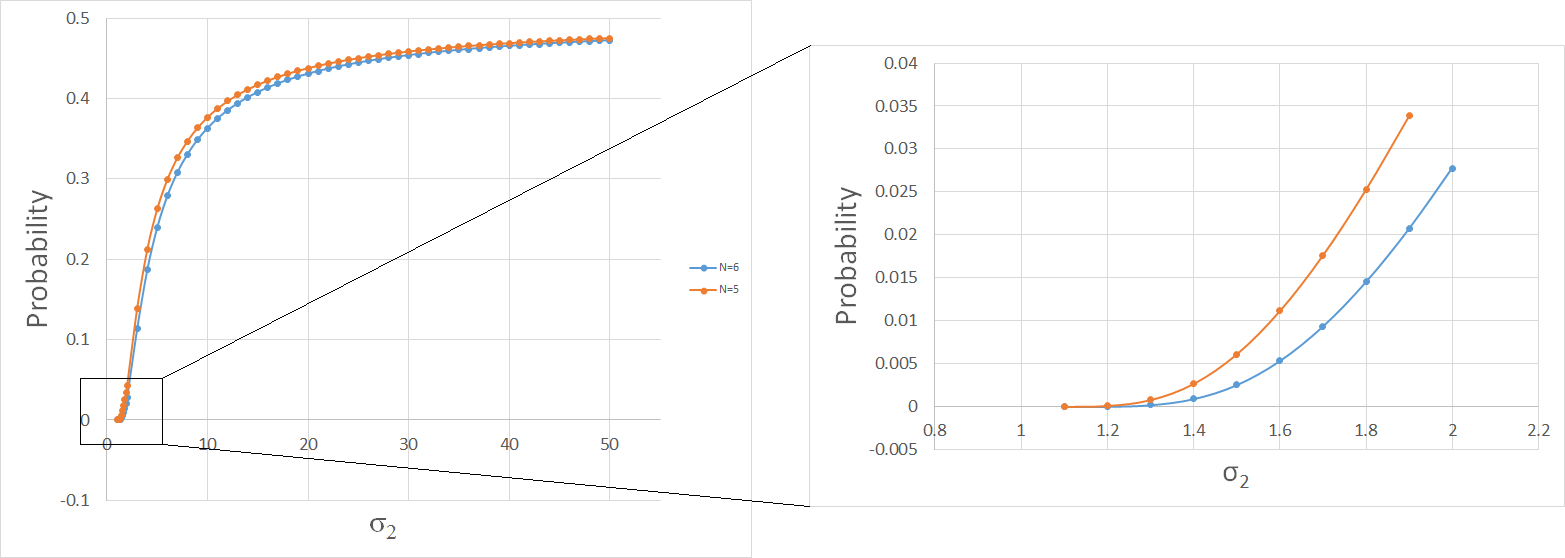
\includegraphics[width=\linewidth]{N6minima.png}
  \caption{The probability that a given extremum with $\phi > 0$ is a minimum as a function of $\sigma_2$, for $N=5,6$. A close-up of the probabilities for small values of $\sigma_2$ is shown as well. The probability for $N=5$ is always larger than that for $N=6$.}
  \label{N6}
\end{figure}

In Fig. \ref{N6}, we present the probability that a given extremum with $\phi > 0$ is a minimum as a function of $\sigma_2$. As expected, if the potential is highly oscillatory (i.e. $\sigma_2$ is large, or $\gamma$ is small), the probability tends towards 0.5 -- equal likelihood of an extremum being a maximum or a minimum. Conversely, if the potential is very smooth ($\sigma_2$ is small), the probability tends towards 0. Further, for any given $\sigma_2$, the probability decreases with increasing dimension.

While this analytical approach works well for low dimensions, the complexity of the integral rises quickly: for illustration, the 4D integral has 15 terms, the 5D integral over 800, and the 6D integral $\sim2800$. To push the results even higher, we switch to numerical integration.

\subsection{$N \leq 10$}
To numerically integrate Eq. \ref{DensityOfPeaks}, we have written a C++ code, using the VEGAS \cite{VEGAS} monte carlo integration routines of the GNU Scientific Library.\cite{GSL} The code is only able to perform the integral for a given value of $\phi$ and $\gamma$. However, with enough data points, it becomes possible to numerically evaluate the probability using the trapezoidal rule. Using $\phi$ in steps of 0.5, we confirm that the numerical integration code matches the analytical integration for $N < 6$ to two digits of precision; we also confirm that agreement improves if we increase the resolution of $\phi$. For example, for $N=4, \sigma_2=3.5$, the exact probability is 0.21005. Comparatively, integrating with the trapezoidal rule with $\phi$ in steps of 0.5 gives a probability of 0.215202; with $\phi$ in steps of 0.1, this changes to 0.210256. This gives us confidence in the numerical results. We present some data up until $N = 10$ in Table 1; beyond $N = 10$, even the numerical integration fails to produce results.

\begin{table}[h!] \label{Data}
  \begin{center}
    \caption{The probability that a given extremum with $\phi > 0$ is a minimum as a function of $\sigma_2$. Values given for $N=4,5,6$ are exact; for larger values they are approximate (see the text; errors are on the order of the third nonzero digit after the decimal).}
    \label{tab:table1}
    \begin{tabular}{c|c|c} % <-- Alignments: center/center/center (l and r for left and right if needed)
      $\textbf{N}$ & $\sigma_2$ & $p_{min}$\\
      \hline
      4 & 10 & 0.60859\\
      5 & 10 & 0.62333\\
      6 & 10 & 0.63680\\
      7 & 10 & 0.35210\\
      8 & 10 & 0.34227\\
      9 & 10 & 0.33159\\
      10 & 10 & 0.32151\\
      \hline
      4 & 3.5 & 0.21520\\
      5 & 3.5 & 0.17886\\
      6 & 3.5 & 0.15274\\
      7 & 3.5 & 0.13599\\
      8 & 3.5 & 0.11711\\
      9 & 3.5 & 0.10093\\
      10 & 3.5 & 0.08729\\
      \end{tabular}
      \quad
      \begin{tabular}{c|c|c} 
      $\textbf{N}$ & $\sigma_2$ & $p_{min}$\\
      \hline
      4 & 2 & 0.066638\\
      5 & 2 & 0.043103\\
      6 & 2 & 0.030844\\
      7 & 2 & 0.02013\\
      8 & 2 & 0.01307\\
      9 & 2 & 0.00845\\
      10 & 2 & 0.00544\\
      \hline
      4 & 1.25 & 0.001526\\
      5 & 1.25 & 0.000327\\
      6 & 1.25 & 6.53328 $\times 10^{-5}$\\
      7 & 1.25 & 2.09673 $\times 10^{-5}$ \\
      8 & 1.25 & 3.97235  $\times 10^{-6}$ \\
      9 & 1.25 & 7.13489  $\times 10^{-7}$ \\
      10 & 1.25 & 1.20253  $\times 10^{-7}$ \\
     \end{tabular}
  \end{center}
\end{table}

As can be seen, the probability that a given extremum with $\phi > 0$ is a minimum decreases with increasing $N$. For a constant $\sigma_0$ and $\sigma_1$, the probability also decreases for increasing $\sigma_2$. Both of these general trends are to be expected: as $N$ increases, there are more conditions that must be simultaneously met for a point to be a minimum, hence the probability decreases. Also, since $\sigma_2$ is the average of the second derivative of the field, as $\sigma_2$ increases the field gets more and more turbulent. This means there are both more maxima and more minima, and the probability decreases.

\subsection{$N > 10$}
For $N > 10$ we have to rely on extrapolation from the lower-dimension case. We have tried two ways to do this.

The first way is to extrapolate from the data in Table \ref{Data}. In Fig. \ref{Log-Linear}, we present a log-linear plot of the probability against the dimension for the three values of $\sigma_2$. The resulting lines are surprisingly straight. There is a noticeable kink in both the $\sigma_2 = 3.5$ and $\sigma_2=2$ case between $N=6$ and $N=7$. This is a numerical effect -- it is where the exact results end and the numerical ones begin. We checked this by running the numerical integration for $N=6$ as well. Replacing the exact result with the numerical one, the kink moves to the left. The kink indicates that the numerical results are consistently overestimating the true probability, but that is not surprising because the numerical results rely on the trapezoidal rule. The trapezoidal rule overestimates the result when the integral is concave up, and underestimates it when it is concave down. The final probability is the area under the curve for $\phi > 0$ divided by the area under the curve for all $\phi$. From Fig. \ref{Likelihood}, for $\phi > 0$ the curve is concave up, so the trapezoidal rule overestimates the numerator, and accordingly the probability as well. This trend holds for higher $N$ as well, since for higher $N$ the plot moves to more negative values.

If the trend is robust, then for the case of $\sigma_2=2$, the probability at $N=100$ is of the order of $p \sim 10^{-42}$. Since there are $\sim 10^{500}$ stationary points in the landscape,\cite{Douglas} this probability, while small, still leads to there being $\sim 10^{458}$ minima that might correspond to our universe.

\begin{figure} 
  \centering
  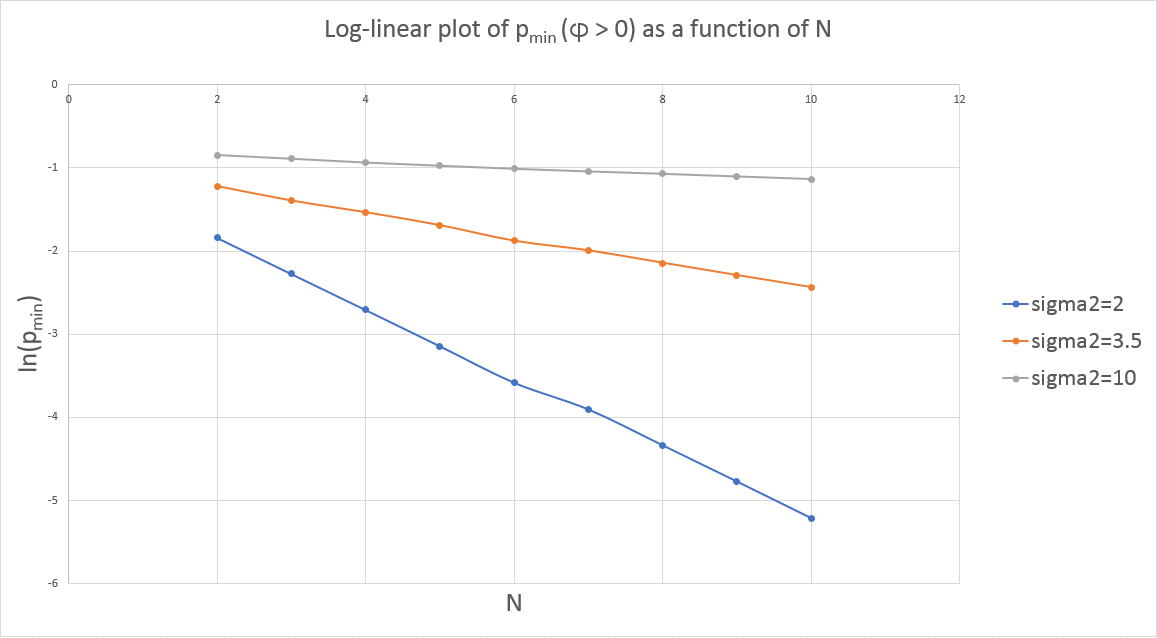
\includegraphics[width=\linewidth]{Log-linear.png}
  \caption{A log-linear plot of the probability that a given extremum with $\phi > 0$ is a minimum for a given $\sigma_2$, as a function of the number of dimensions $N$.}
  \label{Log-Linear}
\end{figure}

\begin{figure}
  \centering
  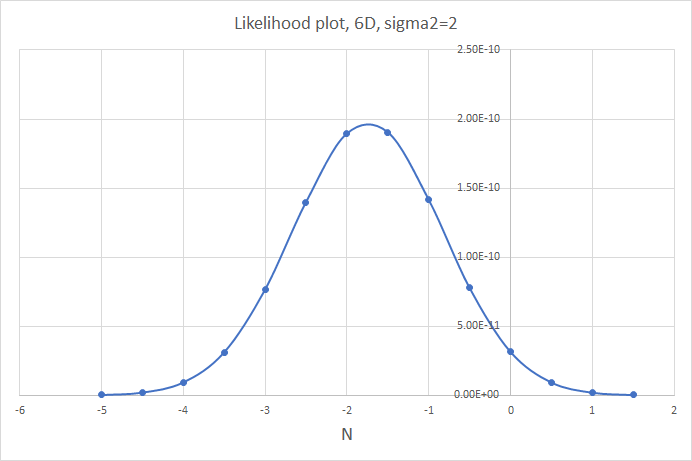
\includegraphics[width=\linewidth]{LikelihoodPlot.png}
  \caption{A plot of the likelihood for $\sigma_2=2, N=6$. The final probability desired is the area under the curve for $\phi > 0$ divided by the area unde the curve for all $\phi$. For the region $\phi > 0$, the curve is concave upwards, so the trapezoidal rule overestimates its value. Accordingly, the numerator and probability are also overestimated.}
  \label{Likelihood}
\end{figure}

The other way is to with ratios of the peak likelihood. The idea is to take the logarithm of the integrand in Eq. \ref{DensityOfPeaks}, which results in a function $G(x, y, z, \ldots)$, and then find the values of $x, y, z \ldots$ which maximizes this integrand. This corresponds to the single most likely point. Having done this, we can compute the ratio of this maximum vs. the point $\phi = 0$. The result in 4D is show in Fig. \ref{LogRatioNoFit}. It's obvious that the blue line is not a good fit of the orange line, but it takes the same shape. Since string theory predicts a truly gargantuan number of stationary points -- on the order of $10^{500}$ -- being off by even $\sim100$ orders of magnitude is not necessarily fatal.

\begin{figure}
  \centering
  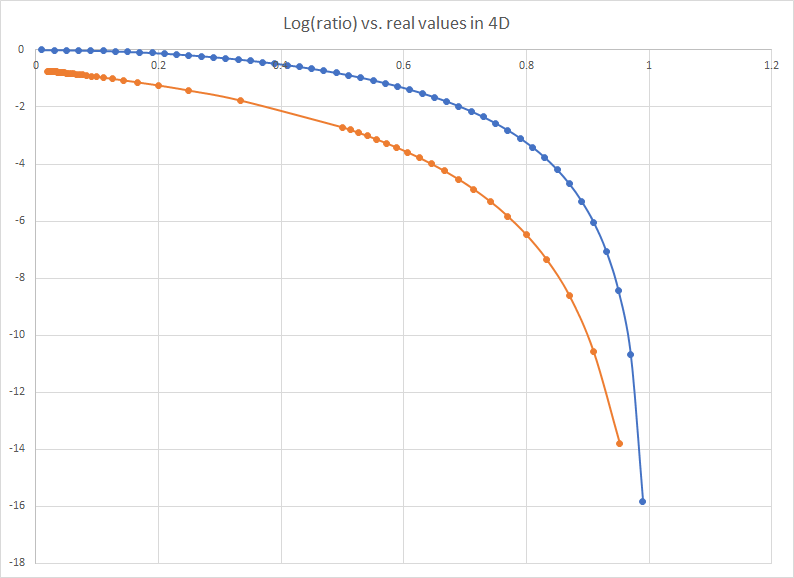
\includegraphics[width=\linewidth]{LogRatioNoFit.png}
  \caption{Plot of the logarithm of the ratio of likelihood for the overall peak to the point $\phi = 0$ as a function of $\gamma$, as well as the analytic results, in 4 dimensions. The blue line is the logarithm of the ratio of likelihood, the orange line is the analytic results.}
  \label{LogRatioNoFit}
\end{figure}

\section{Implications for Multiverse Cosmology}

\re{I would move from looking at the abstract problem in the previous section to the specific implications for cosmology in this section; and how $P(\Lambda)$ depends on $\sigma_2$}

\section{Conclusion}
We have presented results for the statistics of stationary points at a given field value as a function of $N$ and $\sigma_2$. The numbers confirm the intuitive expectation that the probability of a given extremum with $\phi > 0$ being a minimum decreases as $N$ increases or when $\sigma_2$ decreases. We also present a first estimate for the probability at $N=100$ for the $\sigma_2=2$ case, $p \sim 10^{-42}$. However, reliable results are only available up to $N=10$. To push these results up to even greater $N$ is the next goal.

\section{Appendix}
For $N=4$, the full form of the integral Eq. \ref{DensityOfPeaks} is:

\begin{equation}
\begin{split}
N = \frac{1}{214990848} \mathrm{Exp}\frac{9x^2\sigma_1^4 + 2\nu x \sigma_0 \sigma_1^2 \sigma_2 - (v^2+10x^2)\sigma_0^2\sigma_2^2}{-2\sigma_1^4+2\sigma_0^2\sigma_2^2}\\\bigg{(}80x - 1610e^{3x^2}+128x^3+418e^{3x^2}x^3+4e^{4x^2}\sqrt{\pi}(3+48x^2+64x^4)\mathrm{Erf}[\sqrt{\frac{3}{2}}x]\\
-486e^{\frac{9x^2}{2}}\sqrt{6\pi}x^2\mathrm{Erf}[\sqrt{\frac{3}{2}}x]+81e^{\frac{9x^2}{2}}\sqrt{6\pi}x^4\mathrm{Erf}[\sqrt{\frac{3}{2}}x]\bigg{)}
\end{split}
\end{equation}

The higher-dimensional results take the same form: an overall exponential multiplied by a product of polynomials and error functions; however they are massive (for 5D for example, there are some eight hundred terms).

\begin{thebibliography}{99}
\bibitem{Planck2018} Planck Collaboration 2018 results. Submitted to \emph{Astronomy \& Astrophysics}.
\bibitem{DES} Dark Energy Survey year 1 results. arXiv:1802.05257
\bibitem{Linde1986} A. D. Linde, Phys. Lett. B 175, 4, 395--400, 1986
\bibitem{Adshead2007} P. Adshead, R. Easther, and E. A. Lim, Phys. Rev. D 79, 063504, 2009
\bibitem{Guth2001} A. Guth, arXiv: astro-ph/0101507
\bibitem{Susskind2003} L. Susskind, arXiv:hep-th/0302219
\bibitem{Bousso2000} R. Bousso and J. Polchinski, Journal of High Energy Physics, 06, 006, 2000
\bibitem{Agrawal2018} P. Agrawal, G. Obied, P. J. Steinhardt, C. Vafa, Physics Letters B, 784, 271--276, 2018
\bibitem{GRF1} A. Masoumi, A. Vilenkin and M. Yamada, Journal of Cosmology and Astroparticle Physics, 05:053, 2017
\bibitem{GRF2} A. Masoumi, A. Vilenkin and M. Yamada, Journal of Cosmology and Astroparticle Physics, 12:035, 2017
\bibitem{GRF3} T. Bjorkmo and M.C.D. Marsh, Journal of Cosmology and Astroparticle Physics, 02:037, 2018
\bibitem{Aazami2006} A. Aazami and R. Easther, Journal of Cosmology and Astroparticle Physics (0603:013), 2006
\bibitem{Bray2007} A. J. Bray and D. S. Dean, Phys. Rev. Lett. 98, 150201, 2007
\bibitem{Yamada2018} M. Yamada and A. Vilenkin, Journal of High Energy Physics 2018: 29, 2018
\bibitem{Dean2008} D. S. Dean and S. N. Majumdar, Phys. Rev. E., 77, 041108, 2008
\bibitem{Majumdar2009} S. N. Majumdar, C. Nadal, A. Scardicchio, and P. Vivo., Phys. Rev. Lett., 103, 220603, 2009
\bibitem{Bachlechner2014} T.C. Bachlechner, Journal of High Energy Physics, 2014: 54, 2014
\bibitem{Battefeld2012} D. Battefeld, T. Battefeld, S. Schulz, Journal of Cosmology and Astroparticle Physics, 06:034, 2012
\bibitem{Fyodorov2013} Y. V. Fyodorov, Markov Processes Relat. Fields, 21, 483--51, 2015
\bibitem{Masoumi2017} A. Masoumi, M. Yamada and A. Vilenkin, Journal of Cosmology and Astroparticle Physics, 07:003, 2017
\bibitem{Easther2016} R. Easther, A. Guth and A. Masoumi, arXiv:1612.05224 (2016)
\bibitem{Kac1943} M. Kac, \emph{Bull. Amer. Math. Soc.}, 43, 314–320, 1943
\bibitem{Rice1945}  S. O. Rice, \emph{Bell System Tech. J.}, 24, 46--156, 1945
\bibitem{BBKS} J. M. Bardeen, J. R. Bond, N. Kaiser, and A. S. Szalay, Astrophysical Journal, Astrophysical Journal, vol. 304, page 15-61 (1986)
\bibitem{Goldstein} See e.g. H. Goldstein, C. P. Poole, and J. L. Safko, \emph{Classical Mechanics 3rd ed.}, Pearson (2001)
\bibitem{VEGAS} G. P. Lepage, Journal of Computational Physics 27, 192, 1978.
\bibitem{GSL} B. Gough, \emph{GNU Scientific Library Reference Manual - Third Edition, 3rd ed.} (Network Theory Ltd., 2009).
\bibitem{Douglas} M. R. Douglas, Journal of High Energy Physics, 05:046, 2003
\end{thebibliography}

\end{document}